\chapter{Design Framework}
The portal is implemented using Django framework of python. In Django framework every major section is implemented using apps. These apps has little to no dependency over other apps and can exist independently.

\section{MVC Design Pattern}

\begin{figure}[htp]
\center
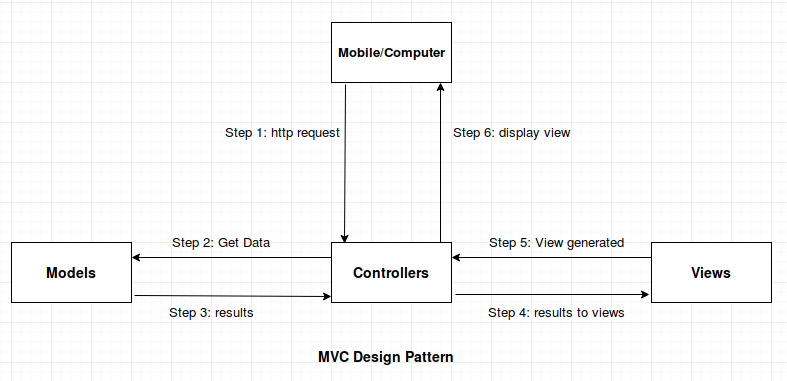
\includegraphics[width=1.0\columnwidth]{mvc}
\caption{MVC Design Pattern}
\label{fig:MVC Design Pattern}
\end{figure}

Model View Controller (MVC) is a software architectural pattern for implementing user interfaces. It divides a given application into three interconnected parts in order to separate internal representations of information from the ways that information is presented to and accepted from the user.The MVC design pattern decouples these major components allowing for efficient code reuse and parallel development.


\section{Django MTV Design Pattern}
According to the Django Book, Django follows the MVC pattern closely enough to be called an MVC framework.Django has been referred to as an MTV framework because the controller is handled by the framework itself and most of the excitement happens in models, templates and views.

\begin{figure}[htp]
\center
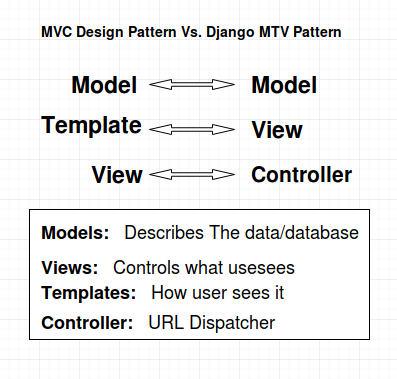
\includegraphics[width=0.5\columnwidth]{mvcMtv}
\caption{MVC Vs Django MTV}
\label{fig:MVC Vs Django MTV}
\end{figure}

\section{Django KodeFork Project}
Django project is a way to develop a web portal using Django framework and python as server side language. For example project \textbf{kodefork} is started using
\begin{minted}
[frame=lines,framesep=2mm,baselinestretch=1.2,]
{python}
django-admin startproject kodefork
\end{minted}

It creates a kodefork project directory. Inside the project directory there is an initial \textbf{kodefork app} and \textbf{manage.py} file.\\

\subsection{kodefork app}
It has mainly \textbf{settings.py} file and \textbf{urls.py} file.
\begin{itemize}
    \item\textbf{settings.py file:} This file contains all the basic settings for the project. It contains setting mainly for:
        \begin{itemize}
            \item Base Directory
            \item Secret Key
            \item Allowed Hosts
            \item Installed Apps
            \item Root URL
            \item Templates
            \item WSGI Application
            \item Databases
            \item Authorization Password Validators
            \item Language Code
            \item Time Zone
            \item Static Root and Static URL
            \item Media Root and Media URL
            \item Accounts
            \item Emails
        \end{itemize}
        
    \item\textbf{urls.py file:}This file contains starting urls for all apps. After start of url is matched, it then calls the urls.py of that particular app to handle subsequent request.For example:
    \begin{minted}
    [frame=lines,framesep=2mm,baselinestretch=1.2,]
    {python}
    # URL Handler for the website
    from django.conf.urls import url,include
    from django.contrib import admin
    admin.autodiscover()   
    urlpatterns = [
        url(r'^admin/', admin.site.urls),    
        url(r'^', include('main.urls')),   
        url(r'^learn/', include('learn.urls')),
        url(r'^questions/', include('questions.urls')),
    ]
    \end{minted}   
    
\end{itemize}

\subsection{manage.py file}
manage.py file is used for carrying management related tasks on the project. After starting project we need to create initial migrations and migrate it to database using:
\begin{minted}
[frame=lines,framesep=2mm,baselinestretch=1.2,]
{python}
# Make initial migrations
python manage.py makemigrations
# Make changes to database
python manage.py migrate
\end{minted}

Above commands creates an automatic admin portal with \textbf{users} model and \textbf{groups} model. This can be viewed by first creating a \textbf{superuser} for this project. For example create super user \textbf{astikanand}:
\begin{minted}
[frame=lines,framesep=2mm,baselinestretch=1.2,]
{python}
# Create Super User
python manage.py createsuperuser
\end{minted}
After Creating superuser start the management server like this
\begin{minted}
[frame=lines,framesep=2mm,baselinestretch=1.2,]
{python}
# In localhost
python manage.py runserver 0.0.0.0:8000
# In live server
Web server runs the project, in this project nginx server
\end{minted}

View the project in browser using:
\begin{minted}
[frame=lines,framesep=2mm,baselinestretch=1.2,]
{python}
# In localhost
http://localhost:8000
# In live server, for this project
http://www.kodefork.com
\end{minted}

\newline
Visit the admin portal now:
\begin{minted}
[frame=lines,framesep=2mm,baselinestretch=1.2,]
{python}
# In localhost
http://localhost:8000/admin
# In live server, for this project
http://www.kodefork.com/admin
\end{minted}

Now to implement any new feature we make an app for it and register it in \textbf{INSTALLED APPS}.

\section{Django Apps}
Every feature in django project is implemented using django apps. An app for example \textbf{ learn app} can be created by
\begin{minted}
[frame=lines,framesep=2mm,baselinestretch=1.2,]
{python}
python manage.py startapp learn
\end{minted}

\textbf{Every app has following items:}
\subsection{migrations directory}
It keeps track of all the migrations or changes that occur on models. After making any change on models inside an app, new migrations are generated using
\begin{minted}
[frame=lines,framesep=2mm,baselinestretch=1.2,]
{python}
python manage.py makemigrations learn
\end{minted}
basically this generates the sql query. After this we need to make changes to database or sync the database with changes. It is done using
\begin{minted}
[frame=lines,framesep=2mm,baselinestretch=1.2,]
{python}
python manage.py migrate learn
\end{minted}
once this is done, we can see that changes get reflected in datatabase model or models.

\subsection{static directory}
It keeps all the static files, like css, js, basic images and serves to the html templates to display pages. Other images and media files are served using Media Server of Django. Static files are served by first including it on top of html file using 

\begin{minted}
[frame=lines,framesep=2mm,baselinestretch=1.2,]
{python}

\end{minted}

and then by making a reference to it

\begin{minted}
[frame=lines,framesep=2mm,baselinestretch=1.2,]
{python}
href=""
\end{minted}


\subsection{templates directory}
It contains all the html files. Once the function inside views.py collects data requested from appropriate model, it send that data to html template file. Inside templates directory basically we have one base.html which is kind of skeleton for every html file. The base.html is inherited on top of every other html file of that app using

\begin{minted}
[frame=lines,framesep=2mm,baselinestretch=1.2,]
{python}

\end{minted}

We make something like containers in base.html file for everything that is to be filled by other html files. For example:

\begin{minted}
[frame=lines,framesep=2mm,baselinestretch=1.2,]
{python}

\end{minted}

In every page we have different content and hence we make container or block for it in base.html file. The data which comes from views to template using a python dictionary is displyed in html file using a template language called \textbf{jinja}

\subsection{urls.py file}
It contains a number of regular expressions to match a url and calls appropriate view function in views.py. For an example

\begin{minted}
[frame=lines,framesep=2mm,baselinestretch=1.2,]
{python}
# URL Handler for the learn
from django.conf.urls import url
from . import views
app_name = 'learn'
urlpatterns = [
    url(r'^$', views.subjects, name='learnhome'),
    
    url(r'^(?P<subjectslug>[A-Za-z-_.]+)/$', views.chapters,
    name='learnsubject'),
    
    url(r'^(?P<subjectslug>[A-Za-z-_.]+)/(?P<categoryslug>
    [A-Za-z-_.]+)/(?P<chapterslug>[A-Za-z-_.]+)/$', 
    views.topics, name='learnchapter'),
    
    url(r'^(?P<subjectslug>[A-Za-z-_.]+)/(?P<categoryslug>
    [A-Za-z-_.]+)/(?P<chapterslug>[A-Za-z-_.]+)/
    (?P<topicslug>[A-Za-z-_.]+)/$',
    views.contents, name='learntopics'),
]
\end{minted}

\subsection{views.py file}
It contains all the views function which controls what user sees, after url make a call to appropriate view function in views.py. The function if necessary collects data from model/models and stores in a dictionary and sends it to appropriate templates file. Templates file after receiving data display it in html using \textbf{jinja} template. For an example

\begin{minted}
[frame=lines,framesep=2mm,baselinestretch=1.2,]
{python}
# Takes a request and send back the response
from django.http import Http404
from django.shortcuts import render,get_list_or_404,
get_object_or_404
from django.db.models import Count
from . models import *

# Get the contents from a particular topic
def contents(request, subjectslug, categoryslug, chapterslug, 
topicslug):

    subject =get_object_or_404(Subject,subjectSlug=subjectslug)
    
    chapter = get_object_or_404(Chapter,subject__subjectSlug=
    subjectslug,chapterSlug=chapterslug)
    
    topics = Topic.objects.filter(subject__subjectSlug=
    subjectslug,category__categorySlug=categoryslug,
    chapter__chapterSlug = chapterslug).order_by('topicNumber')
    
    if not topics:
        raise Http404

    contents = get_object_or_404(Topic, subject__subjectSlug=
    subjectslug,category__categorySlug=categoryslug,
    chapter__chapterSlug = chapterslug,topicSlug=topicslug)

    act = request.path.split('/')[5]
    
    url = '/learn/'+subjectslug+'/'+categoryslug
    
    #create a python dictionary to sent it to html template
    context = { 'subject':subject, 'chapter': chapter, 
    'topics': topics,'contents': contents, 'act':act,
    'url': url }
    
    return render(request, 'learn/contents.html', context)

\end{minted}

We can also write some class based views instead of normal views function. Django also provides some generic class based views.
\begin{itemize}
    \item django.views.generic.ListView
    \item django.views.generic.DetailView
    \item django.views.generic.TemplateView
    \item django.views.generic.edit.FormView
    \item django.views.generic.edit.CreateView
    \item django.views.generic.edit.UpdateView
    \item django.views.generic.edit.DeleteView
\end{itemize}

\textbf{We can use class based views like this.}
\begin{minted}
[frame=lines,framesep=2mm,baselinestretch=1.2,]
{python}
class UserUpdate(LoginRequired,AuthorRequiredMixin,UpdateView):
    model = Profile
    
    template_name = 'users/profile_update.html'
    
    fields = ['gender','profilepic','designation','about',
    'address','website','facebookprofile','twitterprofile',
    'githubprofile','linkedinprofile']
    
    pk_url_kwarg = 'userid'

    def get_success_url(self):
        people = self.get_object()
        
        successurl = '/users/'+str(people.pk)+'/'+
        str(people.user)
        
        return successurl
\end{minted}

The generic views is used to directly create, update or delete entry inside model by creating a form at template specified in it.


\subsection{models.py file}
It contains a collection of models which is same as tables in normal sql language. Every model has several fields denoting entities. For example

\begin{minted}
[frame=lines,framesep=2mm,baselinestretch=1.2,]
{python}
from django.db import models
from ckeditor_uploader.fields import RichTextUploadingField
from django.template.defaultfilters import slugify
from django.core.urlresolvers import reverse
from smart_selects.db_fields import *


# Models for learn section
class Subject(models.Model):
    subjectNumber = models.IntegerField(default=1)
    
    subjectName = models.CharField(max_length=500)
    
    subjectSlug = models.SlugField(editable=False)
    
    subjectDescription = models.TextField(null=True)
    
    subjectKeywords = models.CharField(max_length=500,null=True)
    
    subjectIcon = models.ImageField(upload_to=
    'uploads/learn/%Y/%m/%d/', null=True, blank=True)
    
    subjectThumbnail = models.ImageField(upload_to=
    'uploads/learn/%Y/%m/%d/', null=True, blank=True)
    
    subjectTwitterImage = models.ImageField(upload_to=
    'uploads/learn/%Y/%m/%d/', null=True, blank=True)
    
    subjectOpengraphImage = models.ImageField(upload_to=
    'uploads/learn/%Y/%m/%d/', null=True, blank=True)


    def save(self):
        if not self.id:
            self.subjectSlug = slugify(self.subjectName)

        super(Subject, self).save()

    def __str__(self):
        return self.subjectName
\end{minted}


In above model in \textbf{ImageField} uploadto  is used to a directory as per upload Year, month and date and uploads image, if name conflicts it renames it and then uploads.\textbf{SlugField()} and \textbf{slugify()} function is used to create slug, 
which helps in creating clean urls. For example:\\

\emph{ if subjectname = 'Data Structures' its generated slug will be \\ slug='data-structures'}\\

Once any changes is made in models, new migrations is created and it is migrated to make changes in database as specified earlier.

\subsection{admin.py file}
This file is used to register models inside admin. Once model is registered it shows up in admin panel of project. For example:

\begin{minted}
[frame=lines,framesep=2mm,baselinestretch=1.2,]
{python}
from django.contrib import admin
from .models import Subject, Category, Chapter, Topic

admin.site.register(Subject)
admin.site.register(Category)
admin.site.register(Chapter)
admin.site.register(Topic)
\end{minted}

\subsection{forms.py file}
This file contains all forms related to that app. Forms can be created by 2 types.\\

Firstly by using simple \textbf{forms.form}

\begin{minted}
[frame=lines,framesep=2mm,baselinestretch=1.2,]
{python}
from django import forms

class MessageForm(forms.Form):
    name = forms.CharField(max_length=100)
    email = forms.EmailField()
    subject = forms.CharField(max_length=100)
    message = forms.TextField()
    
\end{minted}

and secondly it can be created using \textbf{forms.ModelForm}

\begin{minted}
[frame=lines,framesep=2mm,baselinestretch=1.2,]
{python}
from django import forms
from . models import Message

class MessageForm(forms.ModelForm):

    class Meta:
        model = Message
        fields = ['name','email','subject','message']
\end{minted}
Form is then processed and saved using appropriate function in views.py.

\section{Working of Django app}
\begin{figure}[htp]
\center
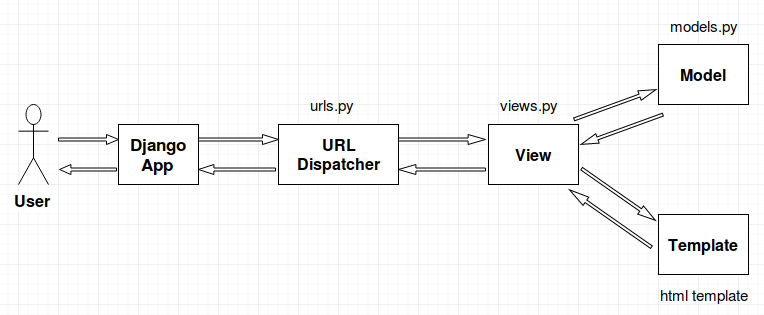
\includegraphics[width=1.0\columnwidth]{djangoapp}
\caption{Working of Django App}
\label{fig:Working of Django App}
\end{figure}

Firstly request made by user using url(regular expression) hits the appropriate django  app, then it checks the urls matching regular expression and then appropriate url is dispatched. The dispatched url calls an appropriate view function in views.py. View function in views.py then collects data from model or models if needed and stores it in a dictionary. It then sends the dictionary to html template file. The data inside the dictionary is displayed in html template file using \textbf{jinja} template. This html file is then displayed to user.\\
\textbf{Almost every feature in django project is implemented using an abstract app and all these apps works in similar fashion as described above.}
